\documentclass[10pt]{article}
\usepackage[a4paper,margin=17mm]{geometry}
\usepackage{graphicx,booktabs,hyperref}
\begin{document}\title{SiPM statistical response: validation pilot}\author{NAUSICAA}\date{}\maketitle
Default: 128 intervals per 250 ns bucket. Maximum saved-event mean-charge difference: 0.0028\%. Measured sensor speedup: 1.7 to 5.7 times. The two-event pilot completed for both gases, including the ASIC stage. Full production remains stopped.

The statistical model preserves binomial PDE and Poisson dark-count sampling. Fixed counts are partitioned into short intervals; finite-cell occupancy gives conditional charge moments. A bounded beta draw supplies charge fluctuations, and the same charge updates recovery. The second recovery moment uses a closure preserving its conditional expected loss. Sparse buckets use individual arrival times and aggregate-state draws. The physical setup has 7,854 cells, 73.4 ns recovery and 250 ns buckets. Synthetic optical cases use PDE = 1 and zero dark rate to isolate response fluctuations; the two additional PDE cases use PDE = 0.30 and 10,000 replicas. Real-event replicas use PDE = 0.30 and the production dark rate, with the same fixed photon input in each replica. The first bb0nu event of each of the four photon files (both gases at E/P = 2.5 and 3) is repeated 256 times. The E/P = 2.5 pure-Xe case is also checked with 512 independent new seeds. Other synthetic cases use 2,000 replicas, except sparse pulses (20,000). The card selects 128 intervals; 32 and 64 measure discretization sensitivity. Error bars show one Monte Carlo standard error. Pilot review budgets are 0.05\% mean discrepancy and 5\% variance discrepancy, or four Monte Carlo standard errors when larger. Covariance uses four standard errors plus 5\% of the neighbouring standard-deviation product. Synthetic table checks evaluate each bucket and its adjacent covariance. Real-event checks evaluate total-event charge; covariance is marked N/A. Plots show total-channel or total-event charge, conditional on fixed photon input. This spread is the sensor contribution, not the full event energy resolution. Sensor-computation speedups use median time per real-event replica; synthetic speedups use the complete ensemble runtime. Feasibility repairs and bounded-variance limiting are counted explicitly.

Independent-seed event check: charge variance ratio = 0.904 +/- 0.084 (one standard error). Detected-count variance / analytical binomial variance: microscopic 1.085 +/- 0.073; statistical 0.952 +/- 0.059. Using the known binomial second moment as a control variate gives charge-variance ratio 0.990 +/- 0.043. The variance estimator subtracts 0.5 times the difference between the sampled squared detected-count deviation from its known mean and its analytical variance. That subtraction has expectation zero; the fixed coefficient is the same for both models. Standard errors come from the per-replica estimator contributions.

At 128 intervals, 90 second-state-moment repairs occurred in 1,445,328,831 aggregate draws; the largest correction to S was 0.1484. Variance-limit adjustments: 0. State repairs adjust the dimensionless second recovery sum S.
\clearpage\noindent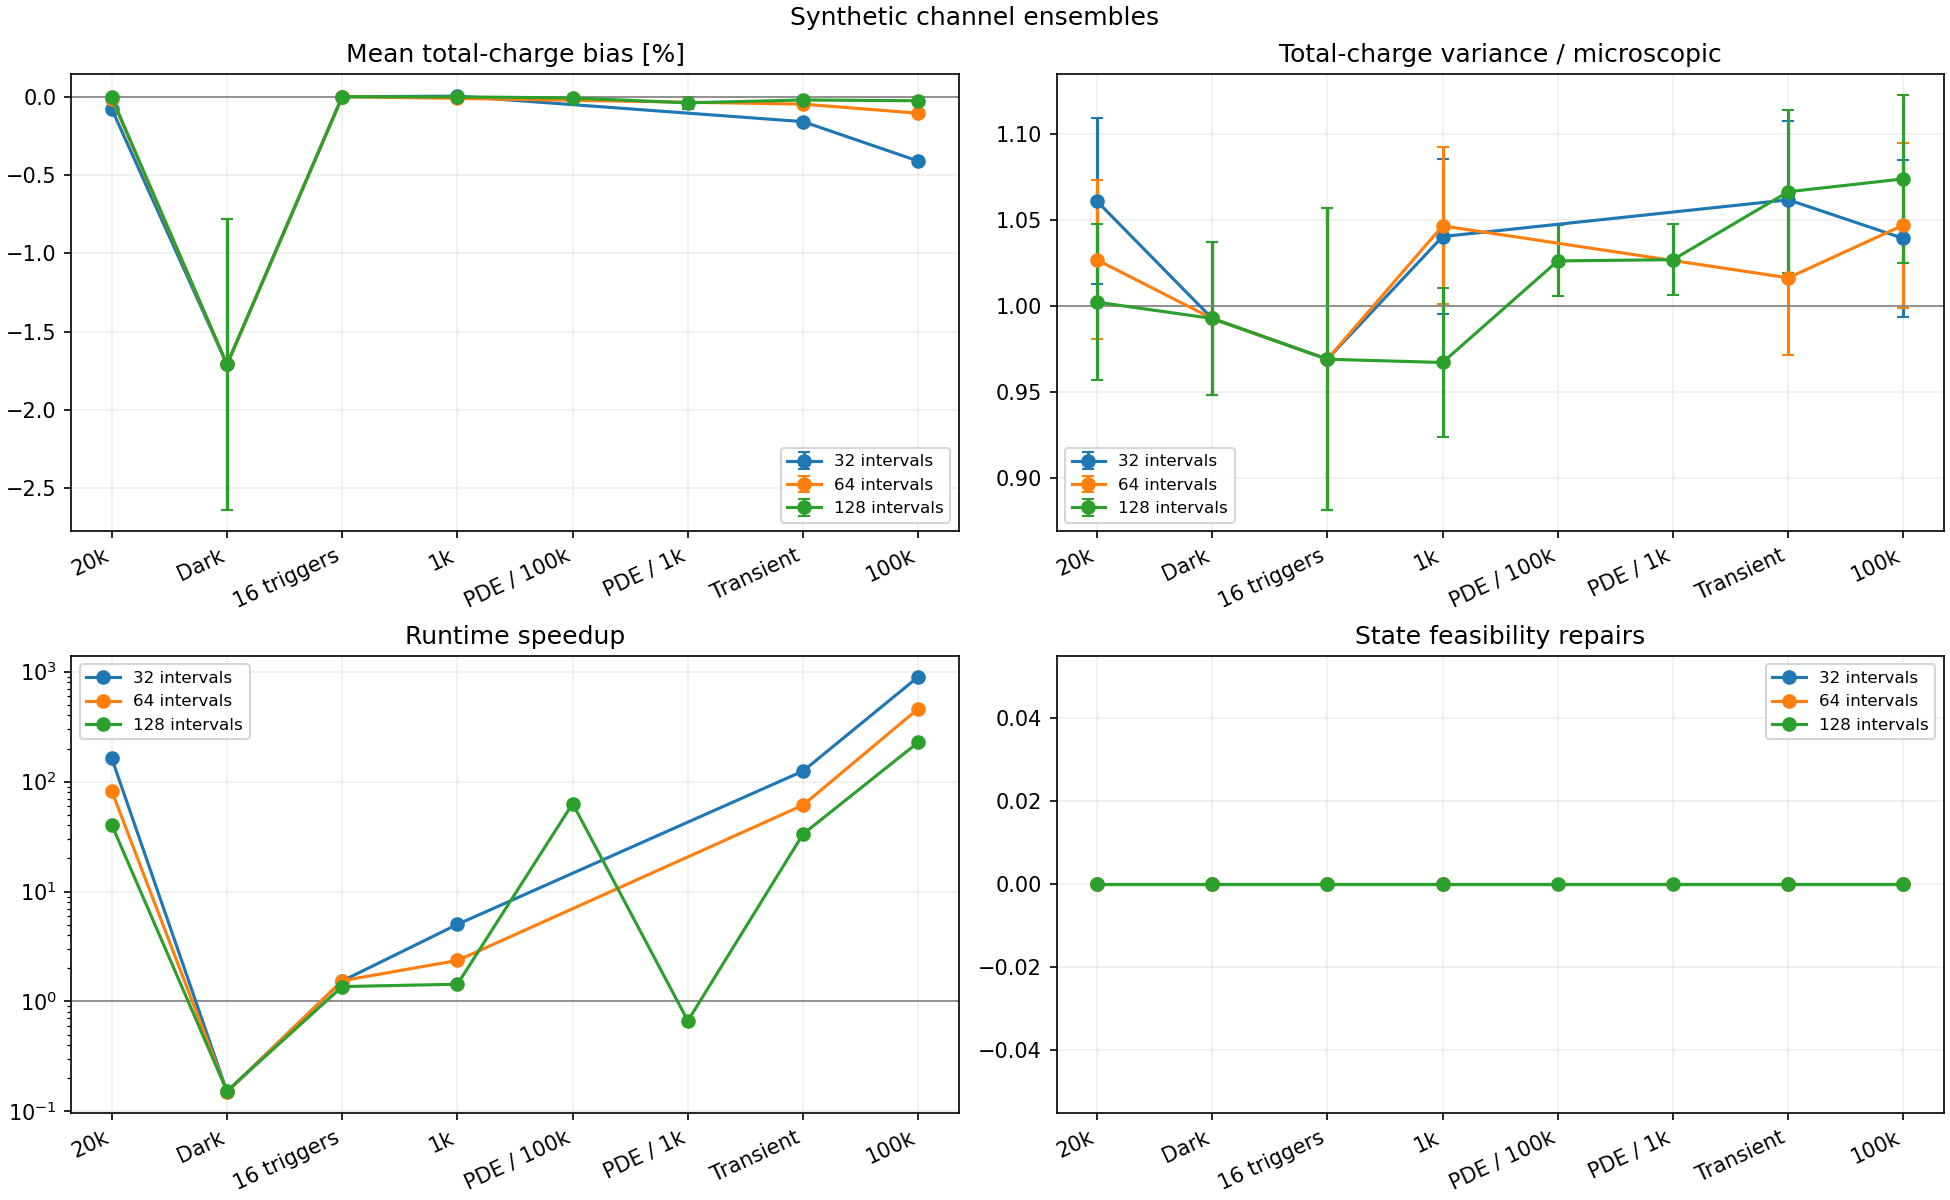
\includegraphics[width=\textwidth]{synthetic_comparison.png}
\clearpage\noindent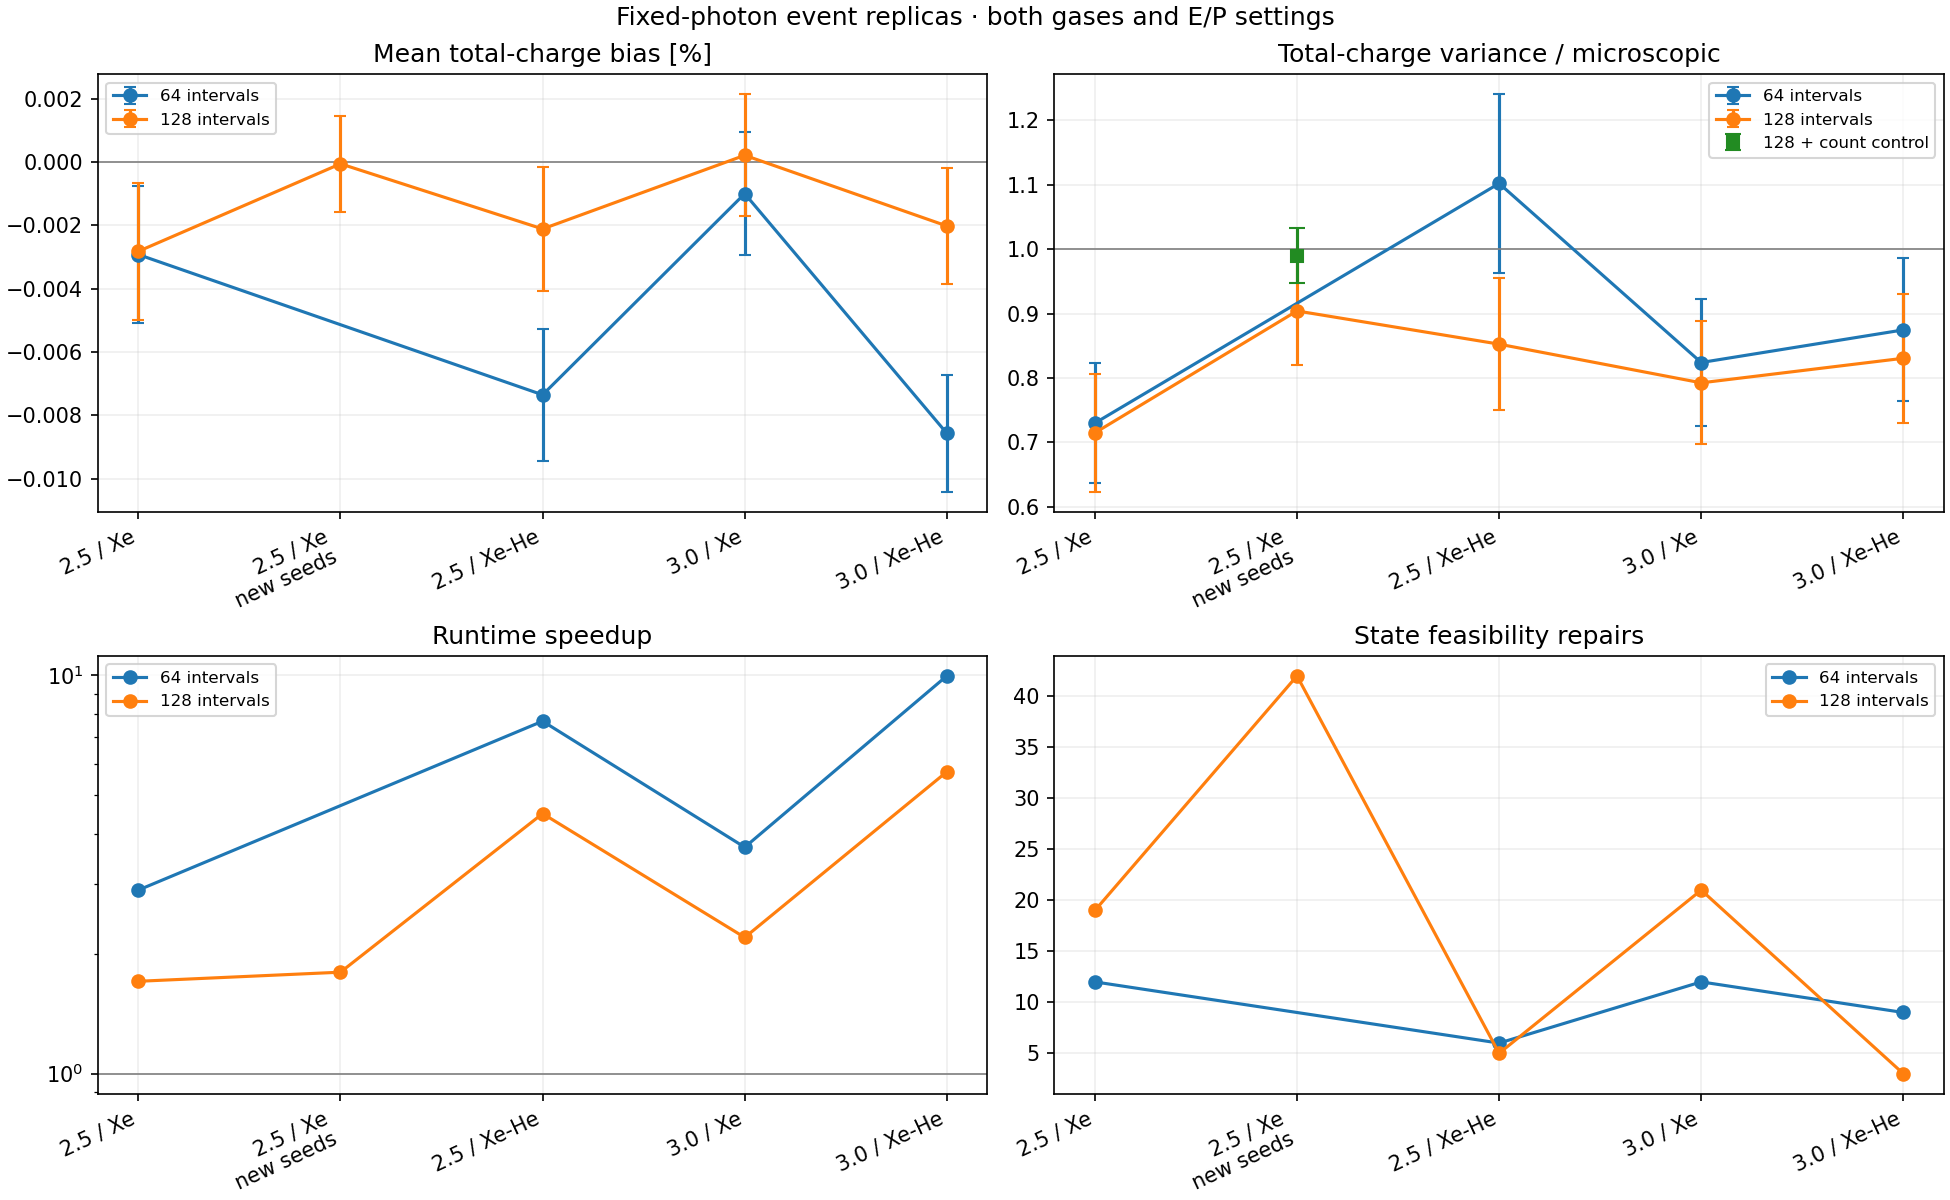
\includegraphics[width=\textwidth]{events_comparison.png}
\clearpage\scriptsize\noindent\resizebox{\textwidth}{!}{\begin{tabular}{lrrrrrrrr}\toprule
Case & Bias (\%) & Var. ratio & Speedup & Mean & Variance & Covariance & Repairs & Limits \\ \midrule
events\_ep2p5\_pure\_xe\_independent\_steps\_128 & -6.023e-05 & 0.9041 & 1.798 & pass & pass & N/A & 42 & 0 \\
events\_ep2p5\_pure\_xe\_steps\_128 & -0.002823 & 0.715 & 1.706 & pass & pass & N/A & 19 & 0 \\
events\_ep2p5\_pure\_xe\_steps\_64 & -0.002926 & 0.7301 & 2.89 & pass & pass & N/A & 12 & 0 \\
events\_ep2p5\_xe\_he15\_steps\_128 & -0.002117 & 0.8526 & 4.497 & pass & pass & N/A & 5 & 0 \\
events\_ep2p5\_xe\_he15\_steps\_64 & -0.007354 & 1.102 & 7.671 & pass & pass & N/A & 6 & 0 \\
events\_ep3\_pure\_xe\_steps\_128 & 0.0002082 & 0.7925 & 2.198 & pass & pass & N/A & 21 & 0 \\
events\_ep3\_pure\_xe\_steps\_64 & -0.001003 & 0.8241 & 3.702 & pass & pass & N/A & 12 & 0 \\
events\_ep3\_xe\_he15\_steps\_128 & -0.002023 & 0.8307 & 5.726 & pass & pass & N/A & 3 & 0 \\
events\_ep3\_xe\_he15\_steps\_64 & -0.00857 & 0.8747 & 9.967 & pass & pass & N/A & 9 & 0 \\
synthetic\_bright\_steps\_128 & -0.001896 & 1.002 & 40.33 & pass & pass & pass & 0 & 0 \\
synthetic\_bright\_steps\_32 & -0.07692 & 1.061 & 162.6 & FAIL & pass & pass & 0 & 0 \\
synthetic\_bright\_steps\_64 & -0.0114 & 1.027 & 81.97 & pass & pass & pass & 0 & 0 \\
synthetic\_dark\_steps\_128 & -1.711 & 0.9927 & 0.153 & pass & pass & pass & 0 & 0 \\
synthetic\_dark\_steps\_32 & -1.711 & 0.9927 & 0.151 & pass & pass & pass & 0 & 0 \\
synthetic\_dark\_steps\_64 & -1.711 & 0.9927 & 0.1501 & pass & pass & pass & 0 & 0 \\
synthetic\_few\_steps\_128 & 0.002137 & 0.969 & 1.366 & pass & pass & pass & 0 & 0 \\
synthetic\_few\_steps\_32 & 0.002137 & 0.969 & 1.536 & pass & pass & pass & 0 & 0 \\
synthetic\_few\_steps\_64 & 0.002137 & 0.969 & 1.545 & pass & pass & pass & 0 & 0 \\
synthetic\_moderate\_steps\_128 & 0.001267 & 0.9671 & 1.435 & pass & pass & pass & 0 & 0 \\
synthetic\_moderate\_steps\_32 & 0.005812 & 1.04 & 5.026 & pass & pass & pass & 0 & 0 \\
synthetic\_moderate\_steps\_64 & -0.008312 & 1.047 & 2.359 & pass & pass & pass & 0 & 0 \\
synthetic\_pde\_bright\_steps\_128 & -0.005608 & 1.026 & 63.11 & pass & pass & pass & 0 & 0 \\
synthetic\_pde\_moderate\_steps\_128 & -0.03709 & 1.027 & 0.6663 & pass & pass & pass & 0 & 0 \\
synthetic\_transient\_steps\_128 & -0.01861 & 1.066 & 33.35 & pass & pass & pass & 0 & 0 \\
synthetic\_transient\_steps\_32 & -0.1573 & 1.062 & 124.8 & FAIL & pass & pass & 0 & 0 \\
synthetic\_transient\_steps\_64 & -0.0453 & 1.016 & 61.15 & FAIL & pass & pass & 0 & 0 \\
synthetic\_very\_bright\_steps\_128 & -0.02377 & 1.074 & 228 & pass & pass & pass & 0 & 0 \\
synthetic\_very\_bright\_steps\_32 & -0.4096 & 1.039 & 899.1 & FAIL & pass & pass & 0 & 0 \\
synthetic\_very\_bright\_steps\_64 & -0.1033 & 1.047 & 461 & FAIL & pass & pass & 0 & 0 \\
\bottomrule\end{tabular}}\end{document}
